\documentclass[conference]{IEEEtran}
\IEEEoverridecommandlockouts
\usepackage{cite}
\usepackage{amsmath,amssymb,amsfonts}
\usepackage{graphicx}
\usepackage{textcomp}
\usepackage{xcolor}
\usepackage{booktabs}
\usepackage{array}
\usepackage{tikz}
\usetikzlibrary{positioning,arrows.meta}

\newcommand{\Meps}{$M(\varepsilon)$}

\begin{document}

\title{Risk-Quantified Virtual Machine Right-Sizing for Private Cloud Capacity Reclamation}

\author{
\IEEEauthorblockN{Abhishek Singh}
\IEEEauthorblockA{Reg. No. 23BCE5044\\
School of Computer Science and Engineering}
\and
\IEEEauthorblockN{Purusharth Kumar}
\IEEEauthorblockA{Reg. No. 23BCE1908\\
School of Computer Science and Engineering}
}

\maketitle

\begin{abstract}
Right-sizing tools report the capacity they reclaim from over-provisioned virtual machines, but not the risk they take on to reclaim it. We build an extreme-value recommender that takes an operator-chosen risk target and returns the smallest catalog flavour expected to meet it, and evaluate it on 792 virtual machines of the Bitbrains GWA-T-12 fastStorage trace against three baselines, under three hypotheses whose thresholds were frozen before any result existed. The evaluation compares methods at matched measured risk, attaches virtual-machine-level bootstrap intervals to every figure, repeats every result on six observation and evaluation splits, and checks the offline violation definition against the kernel on 50 containers replayed under real cgroup limits. All three hypotheses fail. Dominance over the 95th-percentile baseline is not evaluable because the recommender never reaches that baseline's measured risk, calibration is rejected in every scope and split, and zero-risk reclamation is zero. At matched risk the recommender reclaims 2.2 to 6.3 percentage points less than a capped peak baseline, and an ablation attributes its entire gain to a cap at the original allocation rather than to the tail model. The memory violation rule reproduces the kernel verdict on 50 of 50 replayed containers, and the verdicts replicate on a second fleet.
\end{abstract}

%======================================================================
\section{Introduction}
%======================================================================
A virtual machine (VM) in a private cloud is usually sized once, against a peak that someone guessed when it was requested. Fleet studies consistently find that much of that allocation is never used~\cite{qin2023,wacloud2025}. Right-sizing shrinks each VM towards its observed use and returns the difference to the pool, but every unit reclaimed is paid for with headroom: a higher chance that future demand exceeds the new allocation. For memory that event is terminal, because the kernel kills the process; for CPU it throttles the workload. Current tools report the saving and leave this risk unpriced, so an operator cannot tell a safe recommendation from a reckless one that reclaims the same capacity.

This paper asks whether a recommender that prices that risk explicitly reclaims more capacity than simple percentile rules at the same measured risk, and whether its stated risk can be trusted. We make four contributions, each tied to a pre-registered objective: (i) a reproducible offline testbed over a real VM trace, with a flavour catalog, an asymmetric memory/CPU violation definition and three baselines; (ii) \Meps, a recommender built from peaks-over-threshold extreme value theory (EVT) with a clustering correction, that converts a horizon-level risk target $\varepsilon$ into an allocation; (iii) an evaluation protocol that compares methods at matched \emph{measured} risk, attaches VM-level bootstrap intervals to every figure, repeats each result on six splits and ablates every component of the method; and (iv) a kernel-level validation of the offline violation definition on a Kubernetes testbed. Contributions (i) and (iv) evidence objective O1 and (ii)--(iii) objective O2.

The results are mostly negative, and we report them as such. \Meps{} cannot reach the 95th-percentile baseline's risk, it is not calibrated, and it reclaims nothing at zero risk. Where its frontier overlaps a capped peak baseline it reclaims less, and its entire measurable gain comes from a cap the data model imposes. The same protocol also withdrew five of our own interim claims, which we report as corrections.

%======================================================================
\section{Related Work}
%======================================================================
Prior work on VM and container sizing falls into four groups, each of which leaves part of our question open. \emph{Characterisation without a sizing policy} (gap G1) quantifies the gap between allocation and use in private and public clouds~\cite{qin2023,wacloud2025}; Coach exploits temporal patterns to oversubscribe CPU and memory on Azure hosts~\cite{coach2025}, but pools risk at the host rather than exposing it to the owner of each VM. \emph{Forecast-driven recommendation without replay} (G2) attaches conformal intervals to right-sizing recommendations (RSR)~\cite{rsr2025}, sizes instances with a zero-shot foundation model under drift (CLOUDADV)~\cite{cloudadv2026}, or compares deep forecasters on the same GWA-T-12 trace we use~\cite{kollu2024}; none replays an allocation against held-out demand, so exhaustion events go uncounted, and CLOUDADV returns a single operating point with no risk axis. \emph{Uncertainty-aware autoscaling} (G3) treats risk as a constraint, a loss term or a coverage target: MagicScaler~\cite{magicscaler2023}, OptScaler~\cite{optscaler2024}, AQUATOPE~\cite{aquatope2023}, AWARE~\cite{aware2023}, AAPA~\cite{aapa2025} and BACC~\cite{bacc2026}. None states a probability for a decision and checks it against the violations the decision causes, and most scale replicas or sub-second functions rather than a static per-VM flavour over a multi-day window. \emph{Single-answer SLA tuning and production systems} (G4) return one operating point rather than a savings-against-risk curve: Pozdniakova \emph{et al.} search for the one autoscaler threshold that meets an SLA~\cite{pozdniakova2024}, Erms enforces latency SLAs for shared microservices~\cite{erms2023}, Autopilot reports slack and OOM rate as separate outcomes of one tuned policy~\cite{autopilot2020}, and Harvest VMs place the risk on the harvester~\cite{harvest2020}.

Our work combines the pieces these groups hold separately: an operator-chosen risk target, an allocation replayed against held-out demand, a calibration test of the stated risk, and a comparison at matched measured risk. The statistical tools are standard: a Generalized Pareto (GPD) tail above a high threshold~\cite{pickands1975,coles2001}, the extremal index for clustered exceedances~\cite{ferro2003}, the nonparametric bootstrap~\cite{efron1993}, Wilson intervals~\cite{wilson1927} and the expected calibration error (ECE)~\cite{guo2017}.

%======================================================================
\section{System and Data Model}
%======================================================================
\textbf{Trace.} We use the GWA-T-12 Bitbrains fastStorage trace~\cite{shen2015}: one file per VM, 1,250 VMs, samples every 300\,s for 30 days, with provisioned and used CPU and memory in each sample. Each file passes four data-quality gates and is excluded at the first it fails (Fig.~\ref{fig:cascade}): 103 have invalid CPU capacity, 347 fall below the catalog floor (all memory under 2\,GB), 2 change capacity mid-trace and 6 are short. That leaves 792 usable VMs, 425 idle and 367 non-idle, each spanning 30.0 days.

\begin{figure}[t]
\centering
\includegraphics[width=\columnwidth]{fig4_exclusion_cascade.png}
\caption{Data-quality exclusion cascade from 1,250 trace files to 792 usable VMs, one bar per gate in the order the loader applies them. Each VM is counted under the first gate it fails.}
\label{fig:cascade}
\end{figure}

\textbf{Flavour catalog.} Allocations are drawn from a catalog of vCPU $\{1,2,4,8,16\}$ and memory $\{2,4,8,16,32,64\}$\,GB, and every recommendation is snapped \emph{upward} to the next flavour. Without a catalog, right-sizing becomes unbounded continuous shrinking, which no real private cloud permits.

\textbf{Violation definitions.} The two resources are treated asymmetrically, by design. A \emph{memory violation} occurs when demand exceeds the allocation at any single sample, because the process dies. A \emph{CPU violation} requires demand above the allocation for at least two consecutive samples, because contention degrades rather than kills. \emph{Measured risk} is the fraction of VMs with at least one violation in the evaluation window, and \emph{reclamation} is the percentage of vCPU-hours or GB-hours returned relative to the original allocation.

\textbf{Pipeline.} Fig.~\ref{fig:pipeline} shows the path from trace to verdict. Every recommender sees the observation window only; no parameter, threshold or hyperparameter is fitted on the evaluation window. One set of violation functions scores every method, baselines included, and is pinned by unit tests.

\begin{figure}[t]
\centering
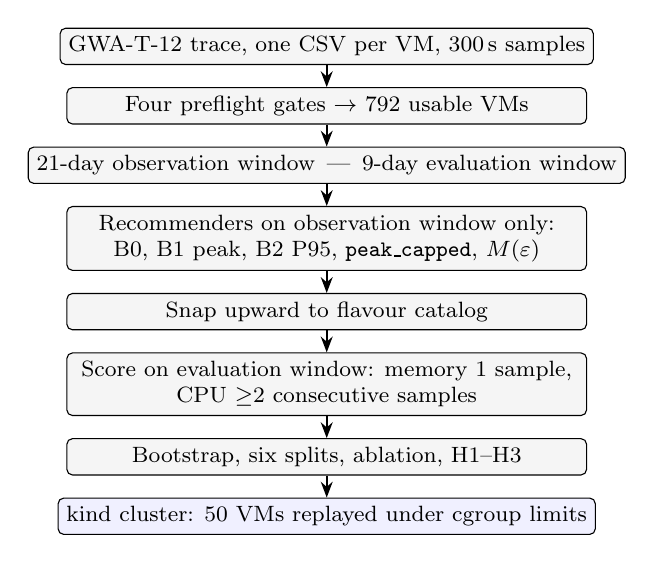
\begin{tikzpicture}[
  node distance=0.28cm,
  box/.style={draw, rounded corners=2pt, align=center, font=\footnotesize,
              minimum width=6.6cm, inner sep=3pt, fill=gray!8},
  arr/.style={-{Stealth[length=2mm]}, thick}]
\node[box] (trace) {GWA-T-12 trace, one CSV per VM, 300\,s samples};
\node[box, below=of trace] (gate) {Four preflight gates $\rightarrow$ 792 usable VMs};
\node[box, below=of gate] (split) {21-day observation window \,|\, 9-day evaluation window};
\node[box, below=of split] (rec) {Recommenders on observation window only:\\ B0, B1 peak, B2 P95, \texttt{peak\_capped}, \Meps};
\node[box, below=of rec] (snap) {Snap upward to flavour catalog};
\node[box, below=of snap] (score) {Score on evaluation window: memory 1 sample,\\ CPU $\geq$2 consecutive samples};
\node[box, below=of score] (stats) {Bootstrap, six splits, ablation, H1--H3};
\node[box, below=of stats, fill=blue!6] (kind) {kind cluster: 50 VMs replayed under cgroup limits};
\foreach \a/\b in {trace/gate,gate/split,split/rec,rec/snap,snap/score,score/stats,stats/kind}
  \draw[arr] (\a) -- (\b);
\end{tikzpicture}
\caption{Evaluation pipeline. Every stage writes its outputs together with the run configuration that produced them.}
\label{fig:pipeline}
\end{figure}

\textbf{Two facts in the trace.} Demand is clipped to the original allocation $a_{\mathrm{orig}}$ on load, so $P(\text{demand} > a_{\mathrm{orig}}) = 0$ for every VM. Upward snapping, meanwhile, pushes the observation peak above $a_{\mathrm{orig}}$ on 210 VMs for memory. Both facts shape the results in Section~\ref{sec:eval}.

%======================================================================
\section{Proposed Method: \Meps}
%======================================================================
For each VM and resource, \Meps{} proceeds in four steps.

\textbf{Tail fit.} Let $u$ be the 0.95 quantile of observation-window demand and $\zeta_u$ the empirical fraction of samples above it. A GPD with shape $\xi$ and scale $\sigma$ is fitted to the excesses over $u$, giving the per-sample probability that demand exceeds a capacity $c$,
\begin{equation}
p(c) = \zeta_u \left(1 + \frac{\xi\,(c-u)}{\sigma}\right)^{-1/\xi}, \qquad c \ge u, \label{eq:tail}
\end{equation}
with the empirical survival function used below $u$, so that $p$ is continuous and non-increasing in $c$. The shape $\xi$ is left unconstrained so that mis-specification shows in the output rather than being hidden, and a VM with too few exceedances falls back to the observation peak, which can only make \Meps{} look worse.

\textbf{Clustering correction.} Extremes in utilisation arrive in bursts, so $n$ samples carry fewer than $n$ independent chances to violate. The extremal index $\theta \in (0,1]$ is estimated with the intervals estimator of Ferro and Segers~\cite{ferro2003}, which has no free parameter; runs declustering at a run length fixed in advance at 12 samples is the sensitivity check.

\textbf{Target conversion.} The operator's target $\varepsilon$ is the probability of at least one violation over the evaluation horizon. With $n_{\mathrm{eval}}$ evaluation samples, derived from the \emph{observation} window's median sampling gap, it becomes the per-sample target
\begin{equation}
p^{*} = 1 - (1-\varepsilon)^{1/(\theta\, n_{\mathrm{eval}})}. \label{eq:target}
\end{equation}

\textbf{Allocation.} \Meps{} returns
\begin{equation}
a(\varepsilon) = \min\Bigl(a_{\mathrm{orig}},\; \min\{c \in \mathcal{F} : p(c) \le p^{*}\}\Bigr), \label{eq:alloc}
\end{equation}
where $\mathcal{F}$ is the flavour catalog. The cap at $a_{\mathrm{orig}}$ follows from the first fact above and was decided before any frontier was computed; the number of capped VMs is reported as a mis-specification diagnostic.

\textbf{Fit diagnostics.} 152 of 652 CPU fits and 41 of 792 memory fits have $\xi \ge 1$, an infinite-mean tail, and CPU falls back to the peak on 140 VMs. The median $\theta$ is 0.251 for CPU and 0.562 for memory, cutting the median effective number of trials from 2,592 to 660 and 1,456.

%======================================================================
\section{Baselines}
%======================================================================
\textbf{B0 (as-provisioned)} keeps $a_{\mathrm{orig}}$ and reclaims nothing. \textbf{B1 (peak)} allocates the observation-window maximum and \textbf{B2 (P95)} its 95th percentile, both snapped upward. Because snapping lifts B1 above $a_{\mathrm{orig}}$ on 210 memory VMs, we add \textbf{\texttt{peak\_capped}}, B1 capped at $a_{\mathrm{orig}}$, which raises peak's memory reclamation from 33.03\% to 41.81\% and is the like-for-like comparator for \Meps, since \Meps{} carries the same cap. Fig.~\ref{fig:baselines} shows the baseline trade-off: P95 reclaims more than peak on both resources and pays for it in safety, most steeply on non-idle VMs.

\begin{figure}[t]
\centering
\includegraphics[width=\columnwidth]{fig2_reclamation_vs_safety_ci.png}
\caption{Reclaimed vCPU, reclaimed memory and share of VMs left violation-free for each baseline and scope. Error bars are 95\% bootstrap CIs over VMs ($B=10{,}000$; $n=792$ all, $n=367$ non-idle).}
\label{fig:baselines}
\end{figure}

%======================================================================
\section{Experimental Setup}
%======================================================================
\textbf{Split and sweep.} Each VM is split by wall-clock time into a 21-day observation window and a 9-day evaluation window. \Meps{} is swept over $\varepsilon \in \{0.001, 0.005, 0.01, 0.05, 0.1, 0.2, 0.4, 0.6\}$, and every point is scored by the same violation functions as the baselines.

\textbf{Uncertainty and replication.} Every reclamation figure, violation fraction, matched-risk gap and ablation shift carries a 95\% percentile bootstrap interval with $B=10{,}000$ resamples of VMs (seed 16). Comparisons are paired: each resample scores every method on the same VMs. When a resampled gap is undefined, because the curves no longer overlap, its share is reported; if it is non-zero the strict interval is withheld and a conditional interval is given instead. Every result is repeated on five further splits (A0--A3 with 14-day observation windows, B7 with 7 days) to cover the axis the bootstrap holds fixed. Proportions use Wilson intervals.

\textbf{Kernel testbed.} Fifty VMs are replayed in five waves as containers on a single-node kind Kubernetes cluster, at a scale of $S=1/16$ with an 80\,MiB margin for the replay agent, and the kernel's OOM kills are compared with the offline prediction.

\textbf{Second fleet.} The full pipeline is re-run unchanged on one month (August 2013) of the GWA-T-12 Rnd trace: 500 files, 316 usable after the same gates.

\textbf{Hypotheses (frozen).} \emph{H1:} at P95's measured risk, \Meps{} reclaims at least 15\% more vCPU-hours and 10\% more GB-hours than P95. \emph{H2:} over $\varepsilon \in \{0.001, 0.005, 0.01, 0.05, 0.10\}$, fewer than 2 measured risks lie outside the 95\% binomial interval of $\varepsilon$, \emph{and} ECE $<0.05$. \emph{H3:} some policy reclaims at least 25\% of vCPU-hours or 20\% of GB-hours with zero violation events. A hypothesis is SUPPORTED only if its statistic clears every clause, NOT SUPPORTED otherwise, and NOT EVALUABLE if the statistic does not exist on the swept range. The thresholds were fixed before the full-fleet run and have not been moved.

%======================================================================
\section{Evaluation}
\label{sec:eval}
%======================================================================

\subsection{Hypothesis verdicts (H1--H3)}
Table~\ref{tab:hyp} gives the headline on the reference configuration (intervals $\theta$, snapped, capped, 21/9 split).

\begin{table*}[t]
\caption{Pre-registered hypothesis verdicts on fastStorage ($n=792$ VMs; non-idle $n=367$). Reference configuration: intervals $\theta$, snapped, capped, 21/9 split.}
\label{tab:hyp}
\centering
\footnotesize
\begin{tabular}{@{}l p{3.2cm} p{2.4cm} p{5.0cm} l p{2.9cm}@{}}
\toprule
& Statistic & Threshold & Measured value & Verdict & Mechanism \\
\midrule
H1 & \Meps{} reclamation at P95's measured risk & $+15\%$ vCPU-h, $+10\%$ GB-h & No matched point: P95 risk 0.0897 CPU / 0.3548 mem; \Meps{} maximum 0.0354 / 0.1187 at $\varepsilon=0.6$ & NOT EVALUABLE & Per-sample targets far more extreme than P95's 1 in 20 \\
H2 & Points outside the 95\% binomial interval; ECE & $<2$ outside; ECE $<0.05$ & CPU 3/5, 3/5; mem 4/5, 4/5 (all / non-idle); ECE 0.025--0.029 & NOT SUPPORTED & Demand leaves the observed range \\
H3 & Largest reclamation with zero violations & 25\% vCPU-h, 20\% GB-h & 0\% (only B0 has zero violations) & NOT SUPPORTED & A minority of VMs violates at any reduction \\
\bottomrule
\end{tabular}
\end{table*}

\textbf{H1 is not evaluable.} At $\theta=1$ and $\varepsilon=0.6$, \eqref{eq:target} gives a per-sample target of $3.53\times10^{-4}$, a 1-in-2,829 quantile. Reaching P95's 1-in-20 would require $\varepsilon = 1 - 1.8\times10^{-58}$, and even at $\theta=0.05$ it would need $\varepsilon=0.9987$. H1 was not reformulated, its comparator was not changed and the sweep was not extended.

\textbf{H2 is NOT SUPPORTED.} The measured-risk curve is much flatter than the target: anti-conservative at low $\varepsilon$ and conservative at high $\varepsilon$. Memory at $\varepsilon=0.001$ measures 0.029 (23 VMs); CPU saturates at 11 VMs for both $\varepsilon=0.05$ and $0.10$. The binomial clause carries the verdict, because the ECE clause cannot reject on this sweep (Section~\ref{sec:threats}). H2 is rejected in all six splits and all four scope/resource cells, with 2 to 5 of 5 points outside the interval, and at $\varepsilon=0.001$ memory risk runs 19 to 30 times the target in every 14- and 21-day split. The pre-registered suspect, serial correlation, is not supported: switching $\theta$ off has no detectable effect (Section~\ref{sec:ablation}).

\textbf{H3 is NOT SUPPORTED.} The nearest misses are \Meps{} at $\varepsilon=0.001$, which reclaims 19.2\% of vCPU-hours with 4 VMs violating and 28.9\% of GB-hours with 23 VMs violating.

\subsection{Comparative frontier at matched risk}
Since H1's comparator is out of reach, we compare against the baseline the frontier does overlap, \texttt{peak\_capped} (Fig.~\ref{fig:frontier}). This comparison is exploratory and is not H1. Each matched point is a linear interpolation between the two bracketing $\varepsilon$ values, and the gap is \Meps{} reclamation minus \texttt{peak\_capped} reclamation at \texttt{peak\_capped}'s measured risk (Table~\ref{tab:gap}).

\begin{figure}[t]
\centering
\includegraphics[width=\columnwidth]{frontier_theta_intervals.png}
\caption{Measured risk against reclamation for \Meps{} ($\varepsilon$ sweep) and the baselines, $n=792$ VMs. Error bars on both axes are 95\% bootstrap CIs over VMs ($B=10{,}000$). Split 21/9, fastStorage.}
\label{fig:frontier}
\end{figure}

\begin{table*}[t]
\caption{\Meps{} minus \texttt{peak\_capped} reclamation at \texttt{peak\_capped}'s measured risk, in percentage points. 95\% paired bootstrap CI ($B=10{,}000$); split columns give the point estimate on the alternative splits.}
\label{tab:gap}
\centering
\footnotesize
\resizebox{\textwidth}{!}{%
\begin{tabular}{@{}l c c c c c c@{}}
\toprule
Cell & \texttt{peak\_capped} risk / reclamation, \% (95\% CI) & Gap & 95\% CI & Undefined share & Splits A0--A3 & Split B7 \\
\midrule
All VMs, CPU      & 0.0164 / 37.70 [33.30, 41.99] & $-5.56$ & $[-11.07, -2.47]$ & 0 & $-6.21$ to $-4.40$ & $-4.85$ \\
All VMs, memory   & 0.0644 / 41.81 [33.34, 49.62] & $-6.30$ & $[-9.18, -3.45]$ & 0 & $-7.09$ to $-2.97$ & $-1.97$ \\
Non-idle, CPU     & 0.0273 / 20.49 [14.42, 26.65] & $-2.15$ & conditional $[-4.02, 0.30]$ & 0.0001 & $-4.70$ to $-1.85$ & $-1.69$ \\
Non-idle, memory  & 0.0708 / 30.97 [15.94, 43.47] & $-3.61$ & $[-5.71, -1.66]$ & 0 & $-4.19$ to $-1.72$ & $-1.00$ \\
\bottomrule
\end{tabular}}
\end{table*}

\Meps{} reclaims \emph{less} than \texttt{peak\_capped} at matched risk. On three cells the interval excludes zero. On non-idle CPU the strict interval is withheld, because the gap is undefined in 1 of 10,000 resamples, and the conditional interval reaches zero. The sign is negative in every split and every cell, but the splits overlap, so this is consistency rather than an interval and does not upgrade the non-idle CPU cell. No \Meps{} point dominates any baseline.

\subsection{Where the gain comes from (ablation)}
\label{sec:ablation}
We change one component at a time and measure the paired shift in the matched-risk gap against the reference arm (Table~\ref{tab:abl}, Fig.~\ref{fig:ablation}).

\begin{table*}[t]
\caption{Paired shift in the matched-risk gap against the reference arm, in percentage points; positive means the change helped. Brackets are 95\% bootstrap CIs; \emph{c} marks a conditional interval, with the undefined share in parentheses where it is large; bold intervals exclude zero.}
\label{tab:abl}
\centering
\footnotesize
\resizebox{\textwidth}{!}{%
\begin{tabular}{@{}l l l l l@{}}
\toprule
Arm & CPU, all VMs & CPU, non-idle & Memory, all VMs & Memory, non-idle \\
\midrule
\texttt{theta\_off} (no clustering correction) & $+0.70$ \emph{c} $[-1.67, 4.61]$ (0.40) & n/a \emph{c} $[-1.14, 0.95]$ (0.87) & $+0.93$ \emph{c} $[-0.33, 3.90]$ (0.012) & $+0.16$ $[-0.79, 0.96]$ \\
\texttt{theta\_runs} (runs declustering) & $+0.35$ $[-0.63, 3.71]$ & $-0.22$ \emph{c} $[-0.94, 1.65]$ & $+0.38$ $[-0.34, 1.56]$ & $+0.28$ $[-0.31, 0.83]$ \\
\texttt{snap\_off}$^{\dagger}$ (no catalog) & $\mathbf{-8.50\ [-13.45, -2.47]}$ & $-3.92$ \emph{c} $[-7.61, -2.04]$ & $\mathbf{+5.47\ [1.80, 9.08]}$ & $+2.54$ $[-3.31, 7.64]$ \\
\texttt{cap\_off} (no cap at $a_{\mathrm{orig}}$) & $\mathbf{-47.03\ [-79.53, -30.62]}$ & $-27.49$ \emph{c} $[-36.91, -12.54]$ & $\mathbf{-67.84\ [-99.14, -34.79]}$ & $\mathbf{-53.44\ [-75.30, -34.17]}$ \\
\texttt{u\_q90} (threshold $q_{0.90}$) & $+1.20$ $[-0.87, 3.66]$ & $-0.72$ \emph{c} $[-2.61, 1.21]$ & $-0.56$ $[-1.80, 1.11]$ & $-1.41$ $[-3.47, 0.01]$ \\
\texttt{u\_q98} (threshold $q_{0.98}$) & $-1.09$ $[-5.01, 2.26]$ & $+1.83$ \emph{c} $[-0.41, 3.56]$ & $\mathbf{+5.26\ [3.40, 7.62]}$ & $\mathbf{+2.26\ [0.76, 3.90]}$ \\
\bottomrule
\multicolumn{5}{@{}l}{\scriptsize $^{\dagger}$The baseline also moves in this arm, so the shift is not directly comparable with the others.}
\end{tabular}}
\end{table*}

\begin{figure*}[t]
\centering
\begin{minipage}{0.49\textwidth}\centering
\includegraphics[width=\linewidth]{ablation_cpu.png}
\end{minipage}\hfill
\begin{minipage}{0.49\textwidth}\centering
\includegraphics[width=\linewidth]{ablation_mem.png}
\end{minipage}
\caption{All seven ablation arms as measured risk against reclamation, CPU (left) and memory (right), $n=792$ VMs; split 21/9, fastStorage. An arm that sits above the reference curve can still be level with it or behind it at matched risk, which is why Table~\ref{tab:abl} reports paired shifts at matched risk rather than reading positions off the curves.}
\label{fig:ablation}
\end{figure*}

\textbf{The cap is the whole gain.} Every \texttt{cap\_off} interval lies at least 12\,pp below zero, and three of the four at least 30\,pp. Without the cap, matched-risk reclamation turns negative ($-32.3\%$ of GB-hours, all VMs): the fitted tail asks for more capacity than the VM ever had. The cap comes from the data model, not from EVT.

\textbf{The dependence correction has no detectable effect} under either estimator; every \texttt{theta\_off} and \texttt{theta\_runs} interval contains zero.

\textbf{The threshold matters on memory only.} Raising $u$ to $q_{0.98}$ adds 5.26\,pp of memory reclamation, while its CPU effect cannot be distinguished from zero. We keep $q_{0.95}$, because choosing $q_{0.98}$ from this table would be fitting on the evaluation window.

\textbf{Snapping.} Removing the catalog widens the CPU gap and narrows the memory gap, although the baseline moves too in this arm. The memory effect is consistent with our baseline-only finding that 17.0\% of the peak-versus-P95 memory gap is catalog quantisation.

\subsection{Offline definition against the kernel}
Compared naively, the memory rule against the recommendation gives 26 true positives, 4 false negatives, 0 false positives and 20 true negatives (Fig.~\ref{fig:t8}). All 4 false negatives lie between the recommendation and the enforced limit (recommendation plus the agent margin), so this testbed cannot adjudicate them. Compared like with like, peak demand against the enforced limit reproduces the kernel's verdict on \textbf{50 of 50 VMs}, which bounds the true mismatch rate below 7.1\% (Wilson 95\%).

\begin{figure}[t]
\centering
\includegraphics[width=\columnwidth]{fig5_t8_validation_ci.png}
\caption{Offline prediction against kernel outcome for the 50 replayed VMs ($n=50$, five waves, $S=1/16$). The like-with-like rule reproduces the kernel's OOM verdict with zero mismatches; the interval on the mismatch rate is Wilson 95\%.}
\label{fig:t8}
\end{figure}

The CPU axis is \emph{not} validated at this scale, and the kernel's own throttle counters show why. Rescoring wave 1 ($n=14$) from each container's \texttt{cpu.stat} reveals an inversion: VM 332 never exceeds its CPU allocation in 2,591 samples yet is throttled in every period of 97.7\% of its sampling slices, while VM 951 exceeds its allocation (213\% of the limit) and is throttled in only 11.4\%. At $S=1/16$ the quota is 6,250\,\textmu s per 100\,ms period, which the agent's own memory-touching and logging work exceeds unaided, and throttle rate correlates more with peak memory demand ($+0.553$) than with CPU demand relative to the limit ($+0.407$). The CPU signal measured the harness, not the workload.

\subsection{Replication on a second fleet}
Table~\ref{tab:rnd} repeats the headline on Rnd with no threshold, gate or setting changed. All three verdicts and the cap finding replicate. The matched-risk deficit replicates in sign on every cell, but on Rnd only the two CPU cells have intervals that exclude zero, so there it is a firmer claim on CPU than on memory.

\begin{table}[t]
\caption{Replication on GWA-T-12 Rnd (August 2013). Reference configuration, same seeds and thresholds.}
\label{tab:rnd}
\centering
\footnotesize
\begin{tabular}{@{}p{3.2cm} l l@{}}
\toprule
Result & fastStorage & Rnd \\
\midrule
Usable VMs & 792 & 316 \\
H1: max \Meps{} vs.\ P95 risk, CPU & 0.035 vs.\ 0.090 & 0.063 vs.\ 0.146 \\
H1: max \Meps{} vs.\ P95 risk, mem & 0.119 vs.\ 0.355 & 0.155 vs.\ 0.399 \\
H2 points outside, CPU / mem & 3/5, 4/5 & 2/5, 4/5 \\
H3 zero-risk reclamation & 0\% & 0\% \\
Gap vs.\ \texttt{peak\_capped}, CPU all & $-5.56$ & $-4.35^{c}$ \\
Gap vs.\ \texttt{peak\_capped}, mem all & $-6.30$ & $-2.85$ \\
\bottomrule
\multicolumn{3}{@{}l}{\scriptsize $^{c}$Conditional interval $[-8.06, -2.13]$.}
\end{tabular}
\end{table}

\subsection{Interim claims withdrawn}
Five claims made at the interim review did not survive the later parts of the protocol. Three were significance errors, each reading a reproducible point estimate as an effect: that switching $\theta$ off is ``marginally ahead'' (every interval contains zero), that $u=q_{0.98}$ is ``inconsistent across resources'' (it improves memory and its CPU effect is indistinguishable from zero), and that the deficit against \texttt{peak\_capped} holds on all four cells (it holds on three). One was a substitution error: a 29-fold memory miscalibration at $\varepsilon=0.001$ was cited as calibration evidence in place of the pre-registered binomial test, which gives the same verdict for a different reason. One was a construction error: ``every low-$\varepsilon$ memory violator drifted'' is true almost by definition, because at $\varepsilon=0.001$ the allocation is at or above the observation peak for all but 1 to 3 VMs. What survives is that exceeding the observation peak is common (30\% to 38\% of VMs on memory) and large (median evaluation-to-observation peak ratio 2.4 to 3.5). The method fails exactly when demand leaves the observed range, which no tail fitted to that range can anticipate.

%======================================================================
\section{Threats to Validity}
\label{sec:threats}
%======================================================================
Table~\ref{tab:threats} summarises the main threats in the four standard categories, with the direction in which each biases the reported results; the full register is in the repository.

\begin{table}[t]
\caption{Main threats to validity and the direction of their bias on the reported results.}
\label{tab:threats}
\centering
\footnotesize
\begin{tabular}{@{}p{1.25cm} p{4.6cm} p{1.5cm}@{}}
\toprule
Category & Threat & Bias \\
\midrule
Construct & CPU violation rule not validated against the kernel at $S=1/16$; demand clipped at $a_{\mathrm{orig}}$ hides its true magnitude above the allocation. & either way \\
Internal & Duplicate zero-demand rows inflate $n_{\mathrm{eval}}$ on 65 VMs; a swept flag could be accepted but silently ignored. & understates \Meps{} \\
External & Both fleets from one provider; one month each; 300\,s sampling hides sub-sample bursts; the Azure trace has no memory series. & unknown \\
Conclusion & Bootstrap covers fleet composition only; splits overlap; the ECE clause has no power on this sweep. & understates uncertainty \\
\bottomrule
\end{tabular}
\end{table}

The most consequential threat is the scope of the bootstrap. It holds the 21/9 split fixed and treats VMs as independent, so a demand shock shared across VMs is not represented. The multi-split analysis covers the split axis, but neighbouring evaluation windows share 74\% of their days, so the spread across splits is a lower bound on split sensitivity, not an interval. The second is the weakness of the ECE clause: a recommender that never violates scores ECE $=\text{mean}(\varepsilon)=0.0332$, inside the 0.05 bound, so only the binomial clause of H2 discriminates. The third is testbed scale: at $S=1/16$ the cluster validates memory enforcement and the timing of violations, but not CPU and not absolute reclaimed capacity, which comes from the full-scale offline run. Every swept parameter now has a test that it changes the output, after an early version of the sweep recorded a threshold flag without applying it.

%======================================================================
\section{Conclusion}
%======================================================================
On 792 VMs of a real private-cloud trace, an extreme-value right-sizing recommender failed all three of its pre-registered hypotheses: it cannot reach the 95th-percentile baseline's risk, it is not calibrated, and it reclaims nothing at zero risk. Where its frontier overlaps a capped peak baseline it reclaims 2.2 to 6.3 percentage points less, and all of its measurable gain comes from a cap at the original allocation that the data model imposes, not from the tail model. The verdicts replicate on a second fleet, and the memory violation definition is validated against the kernel on 50 of 50 replayed VMs. The same protocol withdrew five of our own interim claims, which is the strongest argument for it: matched-risk comparison, intervals that report undefinedness, split sensitivity and kernel validation form a standard that any right-sizing claim can be held to. The natural next step is a recommender that models demand leaving the observed range, for example through drift detection or fleet-level pooling of tails, validated for CPU on a testbed with enough headroom for the replay harness.

\section*{Acknowledgment}
This trace was graciously provided by Bitbrains IT Services Inc.

\begin{thebibliography}{00}
\bibitem{qin2023} Y. Qin \emph{et al.}, ``How different are the cloud workloads? Characterizing large-scale private and public cloud workloads,'' in \emph{Proc. IEEE/IFIP DSN}, 2023.
\bibitem{wacloud2025} ``Towards workload-aware cloud efficiency: A large-scale empirical study of cloud workload characteristics,'' ACM, 2025.
\bibitem{coach2025} ``Coach: Exploiting temporal patterns for all-resource oversubscription in cloud platforms,'' arXiv:2501.11179, 2025.
\bibitem{rsr2025} Majd, Cheng, Pahlevan, and Meinel, ``Right-sizing recommendations (RSR): Cloud workload conformal prediction for VMs in data center operations,'' in \emph{Proc. IEEE/WIC WI-IAT}, 2025.
\bibitem{cloudadv2026} ``CLOUDADV: Decision-aligned instance sizing with zero-shot foundation models under drift,'' arXiv:2606.31470, 2026.
\bibitem{kollu2024} Kollu \emph{et al.}, ``Comparative analysis of cloud resources forecasting using deep learning techniques based on VM workload traces,'' \emph{Trans. Emerging Telecommun. Technol.}, vol. 35, no. 1, e4933, 2024.
\bibitem{magicscaler2023} Z. Pan \emph{et al.}, ``MagicScaler: Uncertainty-aware, predictive autoscaling,'' \emph{PVLDB}, vol. 16, no. 12, pp. 3808--3821, 2023.
\bibitem{optscaler2024} Zou \emph{et al.}, ``OptScaler: A collaborative framework for robust autoscaling in the cloud,'' \emph{PVLDB}, vol. 17, no. 12, 2024.
\bibitem{aquatope2023} Z. Zhou, Y. Zhang, and C. Delimitrou, ``AQUATOPE: QoS-and-uncertainty-aware resource management for multi-stage serverless workflows,'' in \emph{Proc. ASPLOS}, 2023.
\bibitem{aware2023} H. Qiu \emph{et al.}, ``AWARE: Automate workload autoscaling with reinforcement learning in production cloud systems,'' in \emph{Proc. USENIX ATC}, 2023, pp. 315--330.
\bibitem{aapa2025} Zhang \emph{et al.}, ``AAPA: An archetype-aware predictive autoscaler with uncertainty quantification for serverless workloads on Kubernetes,'' arXiv:2507.05653, 2025.
\bibitem{bacc2026} ``BACC: Budget-aware calibration and control for horizontal autoscaling,'' arXiv:2606.20575, 2026.
\bibitem{pozdniakova2024} O. Pozdniakova, D. Mazeika, and A. Cholomskis, ``SLA-adaptive threshold adjustment for a Kubernetes horizontal pod autoscaler,'' \emph{Electronics}, vol. 13, no. 7, 1242, 2024.
\bibitem{erms2023} S. Luo \emph{et al.}, ``Erms: Efficient resource management for shared microservices with SLA guarantees,'' in \emph{Proc. ASPLOS}, 2023, pp. 62--77.
\bibitem{autopilot2020} K. Rzadca \emph{et al.}, ``Autopilot: Workload autoscaling at Google,'' in \emph{Proc. EuroSys}, 2020, pp. 1--16.
\bibitem{harvest2020} P. Ambati \emph{et al.}, ``Providing SLOs for resource-harvesting VMs in cloud platforms,'' in \emph{Proc. USENIX OSDI}, 2020, pp. 735--751.
\bibitem{pickands1975} J. Pickands, ``Statistical inference using extreme order statistics,'' \emph{Ann. Statist.}, vol. 3, no. 1, 1975.
\bibitem{coles2001} S. Coles, \emph{An Introduction to Statistical Modeling of Extreme Values}. London: Springer, 2001.
\bibitem{ferro2003} C. A. T. Ferro and J. Segers, ``Inference for clusters of extreme values,'' \emph{J. R. Statist. Soc. B}, vol. 65, no. 2, 2003.
\bibitem{efron1993} B. Efron and R. J. Tibshirani, \emph{An Introduction to the Bootstrap}. New York: Chapman \& Hall, 1993.
\bibitem{wilson1927} E. B. Wilson, ``Probable inference, the law of succession, and statistical inference,'' \emph{J. Amer. Statist. Assoc.}, vol. 22, no. 158, 1927.
\bibitem{guo2017} C. Guo, G. Pleiss, Y. Sun, and K. Q. Weinberger, ``On calibration of modern neural networks,'' in \emph{Proc. ICML}, 2017.
\bibitem{shen2015} S. Shen, V. van Beek, and A. Iosup, ``Statistical characterization of business-critical workloads hosted in cloud datacenters,'' in \emph{Proc. IEEE/ACM CCGrid}, 2015.
\end{thebibliography}

\end{document}
